\documentclass[11pt]{article}
\usepackage[a4paper,margin=1in]{geometry}
\usepackage{amsmath,amssymb,amsthm,mathtools}
\usepackage{graphicx}
\usepackage{hyperref}
\usepackage{microtype}
\hypersetup{hidelinks}

\newtheorem{theorem}{Theorem}
\newtheorem{lemma}{Lemma}
\newcommand{\ac}{\operatorname{ac}}
\newcommand{\ar}{\operatorname{ar}}
\newcommand{\conv}{\operatorname{conv}}

\title{A universal counterexample to the renorming converse for asymptotic centers}
\author{Run \texttt{fa\_banach\_001}, agent lane 10}
\date{2026-08-12}

\begin{document}
\maketitle

\section*{Source conjecture}

The source is C.~Angosto, M.~C.~List\'an-Garc\'ia, and F.~Rambla-Barreno,
\emph{Continuity properties of sequentially asymptotically center-complete
spaces} \cite{source}, available as
\href{https://arxiv.org/abs/1403.4646}{arXiv:1403.4646} and later published
in RACSAM.

For a bounded sequence $\bar x=(x_n)$ in a real Banach space, it defines
\[
 \ar(\bar x)=\inf_{z\in X}\limsup_n\|x_n-z\|,
 \qquad
 \ac(\bar x)=\left\{z:\limsup_n\|x_n-z\|=\ar(\bar x)\right\}.
\]
Writing $C_n(\bar x)=\{x_m:m\ge n\}$, its tail pseudometric is
\begin{align*}
 d(\bar x,\bar y)=\inf\{\varepsilon>0:{}&\text{for every }n\text{ there is }m
 \text{ such that}\\
 &C_m(\bar x)\subset C_n(\bar y)+\varepsilon B_X,
 \quad C_m(\bar y)\subset C_n(\bar x)+\varepsilon B_X\}.
\end{align*}

Conjecture 3.3 asks whether equality of both asymptotic centers and radii under
\emph{every equivalent renorming} forces $d(\bar x,\bar y)=0$.  The answer is
no in every nonzero Banach space.

\begin{center}
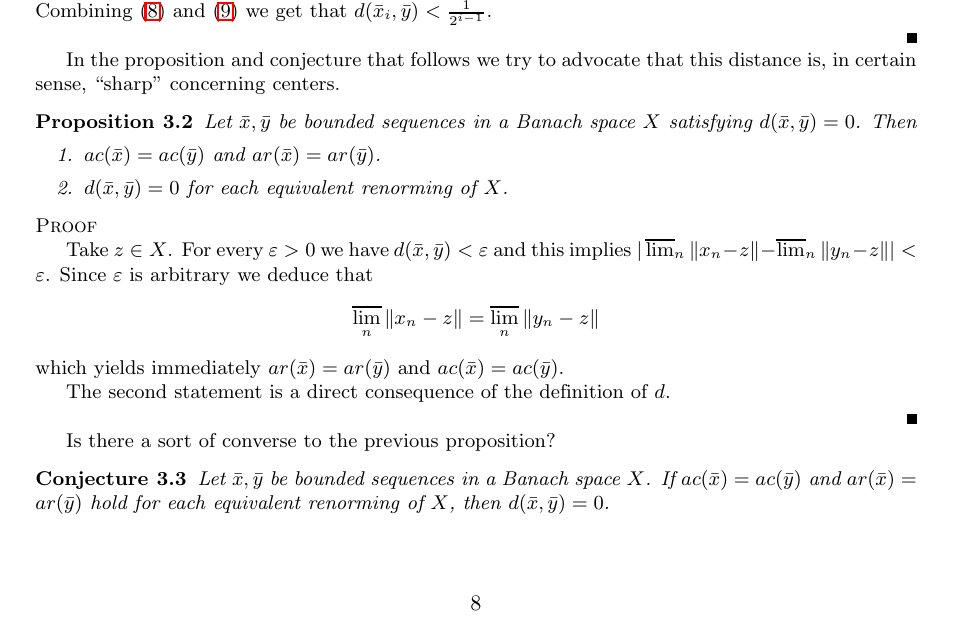
\includegraphics[width=0.95\linewidth]{figures/open_conjecture_crop.png}
\end{center}

\section*{Universal counterexample}

\begin{theorem}\label{thm:counterexample}
Let $X$ be any nonzero real Banach space.  There are bounded sequences
$\bar x,\bar y$ such that, for every equivalent norm $q$ on $X$,
\begin{equation}\label{eq:pointwise}
 \limsup_n q(x_n-z)=\limsup_n q(y_n-z)\qquad(z\in X),
\end{equation}
but
\[
 d(\bar x,\bar y)>0.
\]
In particular, the sequences have the same asymptotic center and radius for
every equivalent renorming, so Conjecture 3.3 is false.  In fact, equality
\eqref{eq:pointwise} is stronger than the conjecture's hypothesis.
\end{theorem}

\begin{proof}
Fix $u\in X\setminus\{0\}$ and take the periodic sequences
\[
 \bar x=(-u,u,-u,u,\ldots),
 \qquad
 \bar y=(-u,0,u,-u,0,u,\ldots).
\]
Let $q$ be any norm on $X$; equivalence to the original norm is not needed for
this part.  For every $z\in X$,
\begin{align*}
 R_x(z)&:=\limsup_n q(x_n-z)=\max\{q(z-u),q(z+u)\},\\
 R_y(z)&:=\limsup_n q(y_n-z)=\max\{q(z-u),q(z),q(z+u)\}.
\end{align*}
Since $2z=(z-u)+(z+u)$, the triangle inequality gives
\[
 q(z)\le\frac{q(z-u)+q(z+u)}2
 \le\max\{q(z-u),q(z+u)\}.
\]
Thus $R_x=R_y$ pointwise, proving \eqref{eq:pointwise}.  Their common radius
is $q(u)$: the triangle inequality applied to
$2u=(z+u)-(z-u)$ gives $R_x(z)\ge q(u)$, while equality holds at $z=0$.
Their common center is therefore
\[
 \{z\in X:q(z-u)\le q(u),\ q(z+u)\le q(u)\}.
\]

Every tail of $\bar x$ has value set $A=\{-u,u\}$, and every tail of
$\bar y$ has value set $B=\{-u,0,u\}$.  Hence the definition of $d$, computed
in the original norm, reduces to the Hausdorff distance between $A$ and $B$.
Since $A\subset B$ and $\operatorname{dist}(0,A)=\|u\|$,
\[
 d(\bar x,\bar y)=\|u\|>0.
\]
This contradicts the conclusion of Conjecture 3.3.
\end{proof}

The one-dimensional instance $X=\mathbb R$, $u=1$ already suffices: the two
periodic value sets are $\{-1,1\}$ and $\{-1,0,1\}$ and their distance is one.
The all-space form shows that the failure is not caused by a shortage of
renormings in dimension one.

\section*{The structural obstruction: convex-hull blindness}

The example is an instance of a general obstruction.

\begin{lemma}\label{lem:hull}
Let $A$ be a finite subset of a normed space.  For every $z\in X$,
\[
 \sup_{a\in\conv A}\|a-z\|=\max_{a\in A}\|a-z\|.
\]
Consequently, periodic sequences enumerating finite sets $A$ and $B$ with
$\conv A=\conv B$ have identical full asymptotic-radius functions under every
norm, although their tail pseudodistance is the Hausdorff distance between
$A$ and $B$ and can be positive.
\end{lemma}

\begin{proof}
If $v=\sum_j\lambda_j a_j$ is a convex combination of points in $A$, then
\[
 \|v-z\|\le\sum_j\lambda_j\|a_j-z\|
 \le\max_{a\in A}\|a-z\|.
\]
The reverse inequality is immediate from $A\subset\conv A$.  For a periodic
sequence, each tail contains its complete finite value set, so the remaining
claims follow directly.
\end{proof}

Here $A=\{-u,u\}$ and $B=A\cup\{0\}$ have the same convex hull.  Thus no
amount of equivalent renorming can make center/radius data recover the
nonconvex tail geometry measured by $d$.  Even replacing the conjecture's
center-and-radius hypothesis with equality of the entire functions
$z\mapsto\limsup_n\|x_n-z\|$ for every equivalent norm would not repair it.

\section*{Verification, novelty, and scope}

The proof is exact and uses only periodic sequences, the triangle inequality,
and the definition of $d$.  The review-critical identities are independently
checkable from the two finite tail sets.  No compactness, center-existence
theorem, or numerical claim is used.

On 2026-08-12, exact-title, exact-conjecture, and exact-renorming-phrase
searches found the arXiv and published source and later work citing the paper
for center-continuity results, but no resolution or correction of Conjecture
3.3.  The four cheap run indexes contained no result for arXiv:1403.4646.
This is a bounded novelty check, not an assertion that every non-arXiv source
has been exhausted.

The result fully refutes Conjecture 3.3 and explains the obstruction through
convex hulls.  It does not address the paper's separate question whether every
codimension-one subspace of a $C(K)$ space is sequentially asymptotically
center-complete.

\section*{Human review recommendation}

Review as a likely-valid full counterexample.  The decisive observation is
pointwise, not merely minimax: adding the midpoint $0$ to the periodic tail set
does not change its farthest-distance function in any norm, while it changes
the tail Hausdorff geometry by exactly $\|u\|$.

\begin{thebibliography}{9}
\bibitem{source}
C.~Angosto, M.~C.~List\'an-Garc\'ia, and F.~Rambla-Barreno,
\emph{Continuity properties of sequentially asymptotically center-complete
spaces}, arXiv:1403.4646; RACSAM \textbf{110} (2016), 809--822.
\end{thebibliography}

\end{document}

